% Chapter 5

\chapter{Reconocimiento del iris} % Main chapter title

\label{Capítulo 5} % For referencing the chapter elsewhere, use \ref{Chapter5} 

%----------------------------------------------------------------------------------------

% Define some commands to keep the formatting separated from the content 
%\newcommand{\keyword}[1]{\textbf{#1}}
%\newcommand{\tabhead}[1]{\textbf{#1}}
%\newcommand{\code}[1]{\texttt{#1}}
%\newcommand{\file}[1]{\texttt{\bfseries#1}}
%\newcommand{\option}[1]{\texttt{\itshape#1}}

%----------------------------------------------------------------------------------------

\section{Introducción}

De todas las etapas de las que se compone un sistema de reconocimiento de iris la extracción de características se puede destacar como la etapa de mayor importancia siendo una de las áreas mas estudiadas dentro de este campo de investigación, pero que aún a día de hoy presenta cuestiones que requieren de estudios adicionales que ayuden a aumentar el grado de robustez y precisión de estos sistemas. Esto hace presentar un nuevo desafío en el reconocimiento del iris en condiciones no ideales, donde las principales tendencias se centran en el estudio relacionado en cuanto a las deformaciones presentadas en la textura y forma del iris. Estas deformaciones son producidas por las degradaciones que sufren las imágenes de iris capturadas en condiciones no ideales que son afectadas por diferentes factores de calidad como iluminación, emborronado, oclusión y perspectiva, entre otros. Este aspecto hace que los sistemas de reconocimiento de iris que son muy dependientes de los detalles de la textura del mismo sean los mas propensos a fallar en las etapas de segmentación y extracción de características, ya que ambas están fuertemente ligadas a dicha textura. Debido a esto, el éxito de acierto en estos sistemas de reconocimiento empeora dando lugar a que se rechacen injustamente a usuarios auténticos por presentar imágenes con mala calidad. \\ \\ 

Hasta el momento, son dos los tipos de aportaciones realizadas en la extracción de características basadas principalmente en los diferentes tipos de representación de la textura del iris: código binario y vector de valores reales. El trabajo de J. Daugman \cite{Reference15} es la base de los métodos basados en el tipo de representación de código binario, a los cuales se les realiza un proceso de codificación de la información de fase de la transformada 2D Gabor wavelets para obtener el código binario debido a que los datos se presentarán como un vector de valores reales una vez realizada la segmentación. Los métodos basados en representación de la información en forma de vector de valores reales utilizan transformaciones similares, aunque mantienen los valores de los resultados originales en forma de vector de valores reales, es decir, no realizan una transformación binaria de los mismos. Será este último tipo de representación en el que se emplee en las pruebas para este Trabajo Fin de Master. \\

Dentro del mismo ámbito, existen 3 principales categorías en las que los métodos de extracción de características pueden ser aplicados: 1) basados en la región del iris completa, 2) basados en regiones de interés y 3) basados en puntos de interés. La primera categoría engloba a los métodos de extracción de características tradicionales los cuales extraen características globales y locales de la región completa del iris. La segunda categoría agrupa los métodos que extraen características locales en regiones de interés con la finalidad de superar la falta de información producida principalmente por oclusiones de párpados y pestañas. Son diferentes las regiones en las que se pueden basar estos métodos tales como: la parte superior de la región normalizada del iris, la región delimitada por el collarete del iris, la región anular del iris antes del proceso de normalización de dicha región, etc. La tercerca categoría incluye los métodos de extracción de características basados en puntos de interés que son detectados en el espacio de escala, sobre los que se extraen vectores de valores reales que describen la apariencia alrededor de cada punto de interés. Estos métodos se componen de un detector de puntos de interés y un descriptor que describe la zona alrededor de cada punto de interés. El empleo de este último tipo de método ha sido muy útil y de gran aporte en aplicaciones de reconocimiento de objetos en imágenes afectadas por problemas de oclusión, objetos amontonados, diferentes fuentes de ruido, etc. Aunque este tipo de método se comporta bastante bien en el caso de imágenes ruidosas, requiere todavía de mejoras en términos de precisión cuando se producen otro tipo de afectaciones en las imágenes. \\ 

Aprovechando las ventajas que aportan los métodos de extracción de características basados en puntos de interés frente al resto, en este Trabajo Fin de Master se va a emplear un método de este tipo de categoría para obtener la información representativa del iris. En definitiva, la finalidad de este Trabajo Fin de Master es la de proponer un nuevo método para la segmentación de iris junto con un nuevo método para la extracción de las características del mismo que se integren un sistema de reconocimiento para mejorar para aumentar la robustez y precisión en el reconocimiento de iris en condiciones no ideales frente a otros sistemas ya existentes. El método de extracción de características del iris propuesto se basa en la combinación de la información obtenida en forma de puntuación desde 3 fuentes de detectores de puntos de interés. Los tres detectores utilizados son: Harris-Laplace \cite{Reference20}, Hessian-Laplace \cite{Reference20} y Fast-Hessian (el detector utilizado por SURF) \cite{Reference21}. Con los puntos de interés localizados por los detectores, se pasa entonces a describir la región alrededor de cada punto de interés a través del descriptor SIFT. De cada una de las fuentes se obtienen las puntuaciones como resultado de comparar imágenes de iris representadas mediante puntos de interés utilizando una distancia propuesta, la cual es una variante restringida de la clásica "proporción de distancias de los vecinos cercanos". Se propone un regla de suma ponderada basada en el ranking de 3 medidas de desempeño (AUC, EER y CRR at Rank-1) para realizar la fusión de las puntuaciones obtenidas mediante las 3 fuentes detectoras de puntos de interés. \\

A través de este nuevo método de extracción de características propuesto se hacen innecesarios los componentes como la segmentación muy precisa del iris o la normalización de la región anular del iris para aumentar el grado de robustez y precisión en el reconocimiento. Este método cuenta con la ventaja de fusionar información de diferentes fuentes, lo cual es una solución eficiente de cara a los problemas prácticos como el ruido en los datos y la no universalidad de los datos entre otros. Se desarrollarán experimentaciones exhaustivas en los modos de verficación e identificación sobre la basa de datos CASIA-IrisV4-Interval para demostrar la validez del método propuesto. \\


%----------------------------------------------------------------------------------------

\section{Descripción del método propuesto}

Para la ejecución del método propuesto de extracción de características del iris basado en puntos de interés es necesario que anteriormente se haya segmentado el iris de la imagen. Para realizar este procedimiento se utilizará el método que se definió en el capítulo 4. Una vez segmentado el iris se le aplicará una mejora de contraste a la textura del mismo para que de esta forma destaquen los puntos mas interesantes de la imagen de cara al método de extracción de características basado en puntos de interés. \\


\subsection{Tratamiento de la textura del iris}

Antes de aplicar el método de extracción de características propuesto sobre la imagen del iris segmentada se realizará un tratamiento a dichas imagenes con el objetivo de mejorar la textura del iris. La aplicación de este procedimiento se realizará a través de un método de mejora de contraste en imágenes popularmente conocido en este ámbito.  Este método es el llamado ecualización de histograma adaptativo por contraste limitado CLAHE (contrast-limited adaptive histogram equalization) el cual tiene como finalidad la de mejorar el contraste en imágenes de escalas de grises \cite{Reference22}.  El modo de operación de CLAHE es aplicado sobre vecindades de 8x8 llamadas ventanas, cuyo propósito es el de mejorar el contraste en cada ventana de manera que el histrograma de la imagen transformada se puede ajustar a un histrograma plano. Del mismo modo, las ventanas vecinas son combinadas utilizando interpolación bi-linear para elminar los bordes incluidos artificialmente. Es importante ajustar el límite del aumento del contraste, ya que en áreas de píxeles homogéneas puede producir una saturación en la imagen. En la siguiente figura se puede ver el resultado de aplicar dicha transformación a la imagen original.\\ \\ \\

\begin{figure}[htbp]
\centering
\subfigure[S1001L01.jpg]{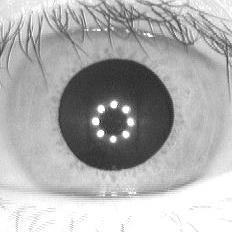
\includegraphics[width=44mm]{tfm-img21}}
\subfigure[S1001L01.jpg]{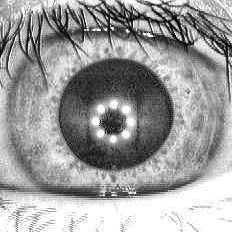
\includegraphics[width=44mm]{tfm-img22}}
\caption{Resultado de la aplicación del método de mejora de constraste CLAHE sobre una imagen de la base de datos CASIA-IrisV4-Internal. (a) Imagen original. (b) Resultado de aplicar el método CLAHE.} \label{fig:señales}
\end{figure}


\subsection{Extracción de las características basada en puntos de interés}

Dentro de los métodos de extracción de características podemos distinguir los que se centran en extraer características locales, normalmente basados en puntos de interés y que presentan un mayor robustez ante problemas de oclusión, objetos superpuestos, diferentes fuentes de ruido y perspectiva, y los métodos que se centran en extraer características globales, los cuales tienen cierta desventaja frente a los anteriores para el reconocimiento de iris en condiciones no ideales. Estos tipos de métodos basados en características globales parten de la desventaja de que no son capaces de diferenciar si un punto o característica pertenece al objeto o al fondo de la escena, requiriendo en estos casos aplicar operaciones adicionales como una segmentación más precisa del iris, lo que resulta bastante complejo en condiciones no ideales. Básicamente, los métodos de extracción de características locales basados en puntos de interés se conforman de un detector de puntos de interés y de un descriptor que describe la región alrededor de cada punto de interés. \\

Los puntos de interés son detectados en el espacio de escala. Para eso nos basamos en el supuesto de que los objetos tienen una propiedad innata en el mundo real por la cual estos sólo existen como entidades con sentido en un cierto rango de escalas. Mediante esta propiedad podemos comprobar como los objetos que son más relevantes en una imagen persisten, y como los menos significativos desaparecen. Para realizar este procedimiento lo que se hace es representar la imagen en múltiples escalas creando para ello un espacio de escala. Este espacio de escala se define como el resultado obtenido de la convolución de una escala variable Gaussiana \textit{G(x, y, z)} con la imagen de entrada \textit{I(x, y)}:\\

\[
L(x,y,\sigma) = G(x,y,\sigma) * I(x,y)
\]

En la siguiente figura se puede ver el efecto de emborronado que produce el cambio brusco de los valores variando el flitro en la función Gaussiana. \\ \\ \\

\begin{figure}[htbp]
\centering
\subfigure[]{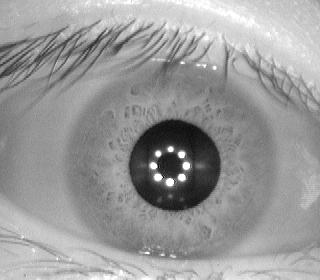
\includegraphics[width=50mm]{tfm-img24}}
\subfigure[]{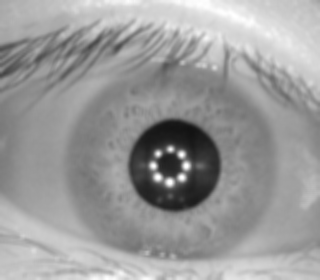
\includegraphics[width=50mm]{tfm-img25}}
\subfigure[]{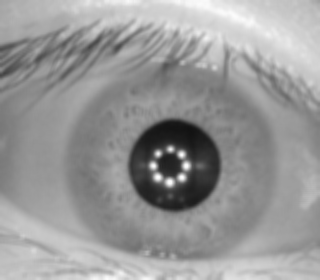
\includegraphics[width=50mm]{tfm-img26}}
\subfigure[]{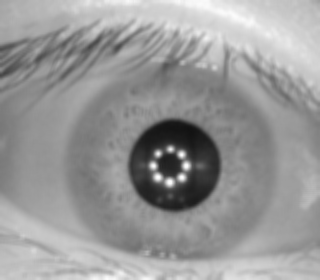
\includegraphics[width=50mm]{tfm-img27}}
\caption{Representación del espacio de escala sobre una imagen de la base de datos CASIA-IrisV4-Internal. (a) Imagen original. (b) $\sigma$ = 3. (c) $\sigma$ = 5. (d) $\sigma$ = 10.} \label{fig:señales}
\end{figure}

Los detectores de puntos de interes se basan en la búsqueda de características tales como esquinas, blobs y regiones dentro de la imagen, identificando en dichos lugares los puntos de interés que no varían en situaciones de transformaciones de escala, perspectiva y/o transformaciones afines. El propósito de los descriptores es el de extraer información discriminante alrededor de los puntos de interés. Estos se clasifican en 3 categorías: basados en distribuciones (SIFT, LJET, FIND, SURF), basados en técnicas de frecuencia espacial (Transformada de Fourier, Transformada de Gabor, Transformada de wavelet) y descriptores diferenciales (Filtros Steerable, Invariante diferencial). \\

El método de extracción de características que se propone en este Trabajo Fin de Master se encuadra dentro de los métodos de extracción de características locales, que como ya se ha visto se componen de un detector de puntos de interés y de un desciptor encargado de describir la región alrededor de cada punto. A diferencia de otros métodos de extracción de características existentes que emplean un único detector de puntos de interés, el método propuesto fusiona 3 detectores dentro del conjunto de los basados en la búsqueda de características en esquinas, blobs y regiones. Para mantener un equilibrio entre los seleccionados de estos tipos de detectores se ha realizado un estudio donde se pueda analizar los resultados que arrojarían utilizando varias combinaciones de estos detectores y descriptores para valorar cual sería la combinación óptima de los mismos \cite{Reference23} \cite{Reference24} \cite{Reference25}. Tras la evaluación investigada sobre las posibles combinaciones de detectores y descriptores, se ha llegado a la conclusión de que el resultado que proporciona un mayor interés en su investigación y que puede ser el más adecuado es el formado por la combinación de los detectores Harris-Laplace (detector de esquina), Hessian-Laplace (detector de blobs) y Fast-Hessian (detector de blobs). Esta combinación de diferentes tipos de fuentes de información evita el poder discriminante que tienen las fuentes individuales en los detectores basados en esquinas que son muy dependientes de una textura bien marcada en controversia con los detectores basados en blobs que son menos dependientes en ese sentido.


\begin{figure}[htbp]
\centering
\subfigure[]{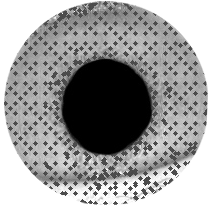
\includegraphics[width=30mm]{tfm-img72} 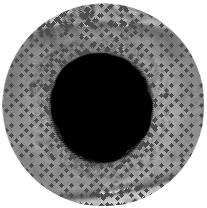
\includegraphics[width=30mm]{tfm-img73} 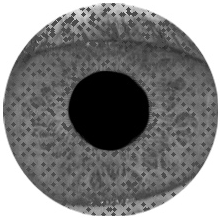
\includegraphics[width=30mm]{tfm-img74}}
\subfigure[]{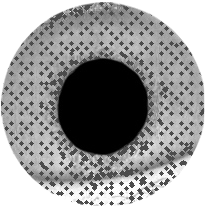
\includegraphics[width=30mm]{tfm-img75} 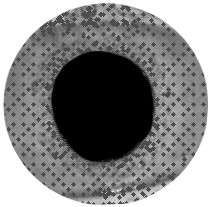
\includegraphics[width=30mm]{tfm-img76} 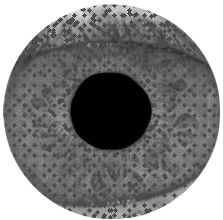
\includegraphics[width=30mm]{tfm-img77}}
\subfigure[]{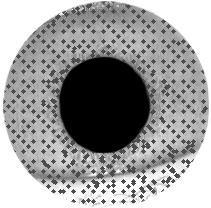
\includegraphics[width=30mm]{tfm-img78} 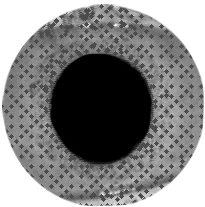
\includegraphics[width=30mm]{tfm-img79} 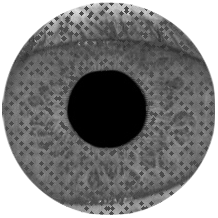
\includegraphics[width=30mm]{tfm-img80}}
\caption{Ejemplos de puntos de interés detectados en instancias de la base de datos CASIA-IrisV4 Internal. (a) Resultados con el detector Harris-Laplace.   (b) Resultados con el detector Hessian-Laplace. (c) Resultados con el detector Fast-Hessian.} \label{fig:señales}
\end{figure}


\subsubsection{Harris-Laplace}

El detector Harris \cite{Reference24} se basa principalmente en la matriz de segundo momento que es definida en la siguiente figura para un punto X.

\[
\mu (X, \sigma_{I}, \sigma_{D}) = \sigma_{D}^{2} g(\sigma_{I}) * \begin{bmatrix}
 L_{x}^{2}(X, \sigma_{D}) &  L_{x} L_{y}(X, \sigma_{D}) \\ 
  L_{x} L_{y}(X, \sigma_{D}) & L_{y}^{2}(X, \sigma_{D})
\end{bmatrix}
\]
\captionof{figure}{Ec. 1.1} 

donde $\sigma_{I}$ es la escala de integración, $\sigma_{D}$ es la escala de diferenciación y $ L_{g}$ es la derivada calculada en la dirección g (X o Y). Esta matriz describe principalmente la distribución del gradiente en un vecindario local de un punto X. Las derivadas locales son calculadas con núcleos (kernel) Gaussianos de un tamaño determinado por la escala local $\sigma_{D}$ (escala de diferenciación). Las derivadas son entonces promediadas entre los vecinos cercanos de los puntos por suavizado con una ventana Gaussiana de tamaño $\sigma_{I}$ (escala de integración). Los valores propios de esta matriz presenta dos cambios principales de señal en los vecinos cercanos de un punto. Basado en esta función, el detector Harris favorece a los pixeles que tienen grandes valores de curvatura en ambas direcciones principales. Por lo tanto, la función de selección es definida como muestra la siguiente figura. 

\[
Harris(X, \sigma_{I}, \sigma_{D}) = \left | \mu (X, \sigma_{I}, \sigma_{D}) \right | - \alpha*trace^{2}(\mu (X, \sigma_{I}, \sigma_{D}))
\]
\captionof{figure}{Ec. 1.2} 

donde $\alpha$ es una constante. En consecuencia, un punto de interés local es identificado donde un pixel alcanza un máximo local con respecto a las esquinas. \\

Para lograr la invarianza de escala, una escala apropiada debe ser elegida para cada punto de interés local detectado. Este proceso implica buscar extremos locales en el espacio de escala. En la matriz del segundo momento adaptada a la escala, el parámetro $\sigma_{I}$ determina la escala de la región local centrada en el punto X. Diferentes $\sigma_{I}$ dan como resultado diferentes máximos locales de función. Sin embargo, no todos los máximos locales generados por diferentes $\sigma_{I}$ son válidos.  Para simplificar el problema, $\sigma_{D}$ está relacionado con $\sigma_{I}$ por un ratio constante, por ejemplo, $\sigma_{D}$ = 0.8 · $\sigma_{I}$ . Como resultado, el problema de buscar parámetros apropiados para $\sigma_{D}$ y $\sigma_{I}$, se ha reducido la búsqueda de extremos locales en el espacio de escala. \\

Sin embargo, como indica T.Lindeberg \cite{Reference26}, la ecuación Ec. 1.2 rara vez alcanza los máximos en el espacio de escala. Por el contrario, si se mide la prominencia de la región con la función Laplaciana de Gauss en el espacio de escala, el extremo local en el espacio de escala puede ser definido con mas precisión.

\[
LoG(X, \sigma_{I}) = \sigma_{I}(L_{xx(x, \sigma_{I})} + L_{yy(x, \sigma_{I})})
\]
\captionof{figure}{Ec. 1.3} 

donde $L_{gg}$ indica la derivada de segundo orden en la dirección g. Como resultado, el detector Harris-Laplace en lugar de medir la prominencia para cada pixel como en la ecuación Ec. 1.2 solo, la Ec. 1.3 es también aplicada en cada pixel. Este proceso ha sido repetido en múltiples escalas. Los puntos de interés finales son localizados en el espacio X-Y donde la ecuación Ec. 1.2 alcanza el máximo local y la ecuación Ec. 1.3 alcanza el extremo local simultáneamente. \\


\subsubsection{Hessian-Laplace}

A diferencia del detector Harris, dada la matriz Hessian para un punto X.

\[
H(X, \sigma) = \begin{bmatrix}
 L_{xx}(X, \sigma) &  L_{xy}(X, \sigma)  \\ 
 L_{xy}(X, \sigma)  &  L_{yy}(X, \sigma))
\end{bmatrix}
\]
\captionof{figure}{Ec. 1.4} 

donde $\sigma$ es el parámetro de suavizado Gaussiano. La ecuación Ec. 1.6 define la prominencia de un punto X únicamente basado en el determinante de la matriz de Hessian. 

\[
H(X, \sigma) = \begin{bmatrix}
 L_{xx}(X, \sigma_{D}) &  L_{xy}(X, \sigma_{D})  \\ 
 L_{xy}(X, \sigma_{D})  &  L_{yy}(X, \sigma_{D}))
\end{bmatrix}
\]
\captionof{figure}{Ec. 1.5} 

De manera similiar a Harris-Laplace, se requiere seleccionar un parámetro $\sigma_{d}$ apropiado. Esto implica la construcción de un espacio de escala con la ecuación Ec. 1.5. Los puntos Hessian son por lo tanto definidos en la ecuación Ec. 1.5 que alcanza los extremos locales en el espacio de escala.. \\

Actualmente, para seleccionar apropiadamente $\sigma_{D}$ en el espacio de escala tenemos otra opción nombrada como la función Laplaciana de Gauss. Si los puntos detectados son requeridos para alcanzar el extremo local con la ecuación Ec. 1.3 en el espacio de escala, se define el nuevo detector Hessian-of-Laplacian. 

\[
H(X,\sigma) = det(H(X,\sigma))  *  \sigma^{4}
\]
\captionof{figure}{Ec. 1.6} 

\begin{table}[htbp]
\begin{center}
\end{center}
\end{table}

\begin{table}[htbp]
\begin{center}
\end{center}
\end{table}

\subsubsection{Fast-Hessian}
Fast Hessian es el detector de características SURF \cite{Reference27}. Su idea básica es calcular la ecuación Ec. 1.6 de una manera eficiente con la ayuda de imágenes integrales. Para permitir un cálculo rápido, la ecuación Ec. 1.6 ha sido aproximada a la ecuación Ec. 1.7.

\[
Det(H_{approx}) = D_{xx}D_{yy} - (0.9D_{xy})^{2}
\]
\captionof{figure}{Ec. 1.7} 

donde $D_{xx}$, $D_{yy}$ y $D_{xy}$ todos pueden ser calculados eficientemente usando filtros de caja. La detección es realizada en cuatro escalas y tres octavos (particiones de tamaño 8). Debido a la considerable pérdida en la aproximación, la localización de los puntos de interés en cualquier espacio de escala o espacio X-Y no puede ser precisa. Parecido al detector DoG, la expansión Taylor en la ecuación Ec. 1.7 es adoptada para aproximar la ubicación exacta de los extremos. En la implementación original de SURF, el detector había sido emparejado con el descriptor SURF por la preocupación existente en cuanto a la velocidad. \\

\subsubsection{SIFT}
Se ha demostrado que el descriptor SIFT tiene éxito en varias tareas tales como clasificación de objetos, generación de panorama e identificación de imagen ND. Dada una región normalizada de un punto de interés, SIFT genera un histograma 2-D en la región local. La región local se particiona en bloques. La figura 5.11 muestra el esquema de partición de SIFT. El gradiente de un píxel dentro de cada bloque de partición se ha cuantificado de acuerdo con su orientación. Normalmente, el número de contenedores de cuantificación es 8 \cite{Reference28}. Antes de la cuantificación, la región local es rotada a su orientación dominante. Esta operación permite que las características extraídas sean invariantes a las transformaciones de rotación. La orientación dominante se estima también en función de la cuantización de la orientación en el campo gradiente de la región local. Generalmente, la región usada para calcular la orientación dominante es una pequeña porción de la región local (por ejemplo, una parte concéntrica de la región local con longitud de radio la mitad). Para lograr un mejor rendimiento, el histograma se pondera adicionalmente en primer lugar	 por su longitud de gradiente, y en segundo lugar por una ventana Gaussiana centrada alrededor del punto de interés. \\

\begin{figure}[htbp]
\centering
\subfigure{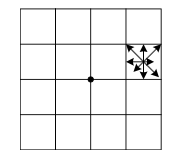
\includegraphics[width=60mm]{tfm-img52}}
\caption{SIFT} \label{fig:señales}
\end{figure}

De entre todos los descriptores mencionados en el estado del arte, se ha seleccionado el descriptor SIFT como el encargado de caracterizar las regiones alrededor de cada punto de interés detectado debido que es el que mejor se integra con los detectores nombrados anteriormente. Además, este descriptor constituye la base de varios descriptores y como se ve en la siguiente figura representa un mayor grado de precisión frente a los demás descriptores. Para reforzar esa decisión se ha analizado el resultado arrojado por una batería de pruebas realizada previamente sobre un conjunto de imágenes de la base de datos CASIA-IrisV4 Internal para cada uno de los 7 descriptores (AOD, ERIFT, FIFT, FIND, LJET, SIFT, SURF) que se mencionaron anteriormente. Se ha utilizado el detector de puntos de interés DoG para este experimento. \\ \\  \\


\begin{figure}[htbp]
\centering
\subfigure{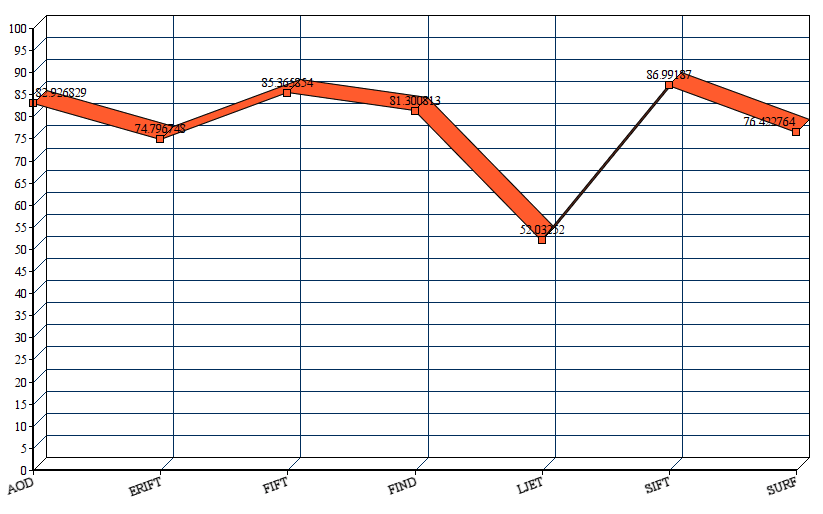
\includegraphics[width=130mm]{tfm-img81}}
\caption{Rendimiento de siete descriptores diferentes con el detector DoG sobre 8 pares de imágenes que cubren transformaciones como escalado, rotación, cambios en el punto de vista, emborronado, cambios en el ratio de comprensión JPEG y cambios de iluminación.} \label{fig:señales}
\end{figure} 


\subsubsection{Comparación de las características}
Con el descriptor que proporcionará las características sobre cada punto de interés ya establecido, ahora toca fijar que tipo de medida se va emplear para clasificar una imagen de iris de prueba como instancia de la clase X. Uno de los métodos más útiles en este ámbito para calcular las similitudes entre 2 imágenes representadas a través de descriptores es la proporción de distancias entre los mismos. De este modo,  para cada punto de interés de una imagen A se calcula la distancia de su descritpor con cada uno de los descriptores de los puntos de interés de una imagen B. \\ \\

\begin{figure}[htbp]
\centering
\subfigure{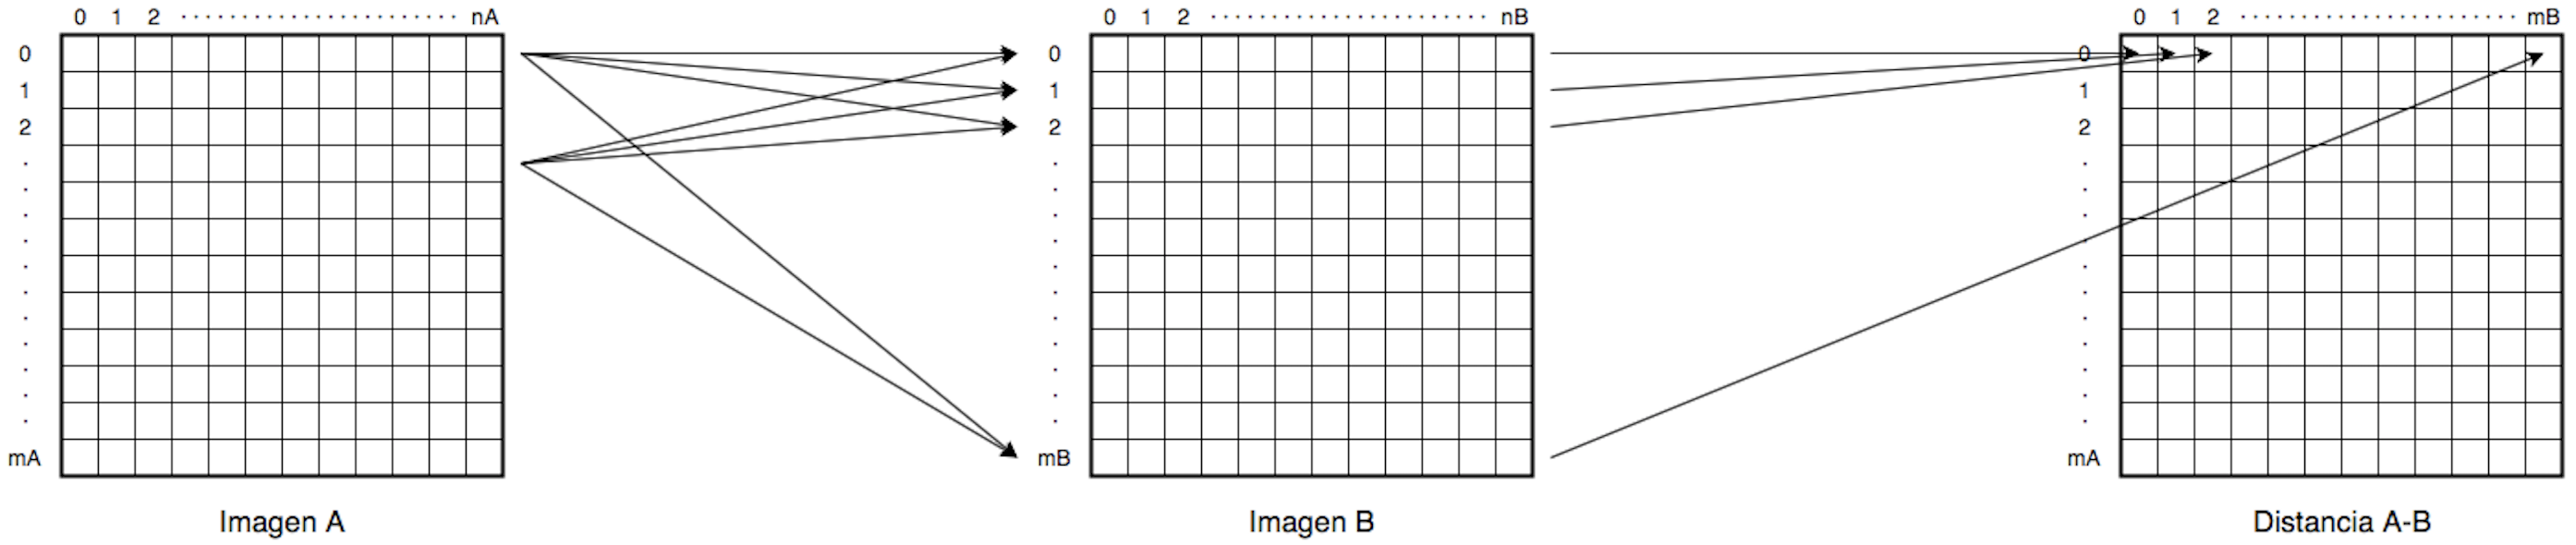
\includegraphics[width=160mm, height=40mm]{tfm-img82}}
\caption{Método para calcular la distancia entre cada punto de interés de dos imágenes representados a través de descriptores.} \label{fig:señales}
\end{figure} 

En la imagen anterior encontramos la representación de la imágenes A y B mediante los descriptores de sus puntos de interés. La \textbf{imagen A} está representada por la estructura de datos de dimensión \textbf{mA} x \textbf{nA}, donde \textbf{mA} es el número de puntos de interés encontrados en dicha imagen por el correspondiente detector, y \textbf{nA} es el número de características halladas para cada punto de interés por el descriptor. De igual manera, la \textbf{imagen B} se representa por la matriz con dimensiones \textbf{mB} x \textbf{nB}, con \textbf{mB} como número de puntos de interés encontrados en la imagen B, y \textbf{nB} la cantidad de características descritas para cada uno de esos puntos de interés. Como salida se obtiene la matriz resultante de dimensión \textbf{mA} x \textbf{mB} que contiene la distancia entre cada uno de los puntos de interés de las dos imágenes.  \\ \\

En el esquema propuesto en la figura anterior se propone un método para el cálculo de la proporción de distancias entre los descriptores de dos imágenes basado en un algoritmo de fuerza bruta. Es decir, para cada punto de interés de la imagen A se calcula la distancia con cada uno de los puntos de interés de la imagen B, obteniendo como resultado una estructura de datos con dimensiones \textbf{mA} x \textbf{mB}. En situaciones como esta en la que nos encontramos con 122 imágenes para clasificar y 1.212 imágenes de prueba, se generarían 147.864 resultados de calcular las distancias entre cada una de las imágenes a clasificar con las imágenes de prueba. Si a esto le sumamos que las imágenes de la base de datos deben ser de una buena calidad y por consiguiente de un mayor tamaño,  el coste computacional que obtendríamos para generar esos resultados sería muy elevado, lo que se traduce en una computadora de características media como una larga espera. \\

Para comprobar el coste computacional que conllevaría este método propuesto, se ha realizado una batería de pruebas sobre un subconjunto del 20\% de imágenes de la base de datos empleada CASIA-IrisV4-Interval. Se ha utlizado DoG como detector de puntos de interés y SIFT como el descriptor para las propiedades de esos puntos de interés. El ordenador en el que se ha realizado la prueba consta de unas características basadas en un procesador Intel Core i5 a 2 GHz, 8 GB  de memoria RAM LPDDR3 a 1867 MHz y un disco duro con una capacidad de 256 GB SSD. \\

Finalizada la experimentación, el tiempo empleado para este escenario ha sido de \textbf{9 minutos y 18.485 segundos} como se muestra en la siguiente figura. \\

\begin{figure}[htbp]
\centering
\subfigure{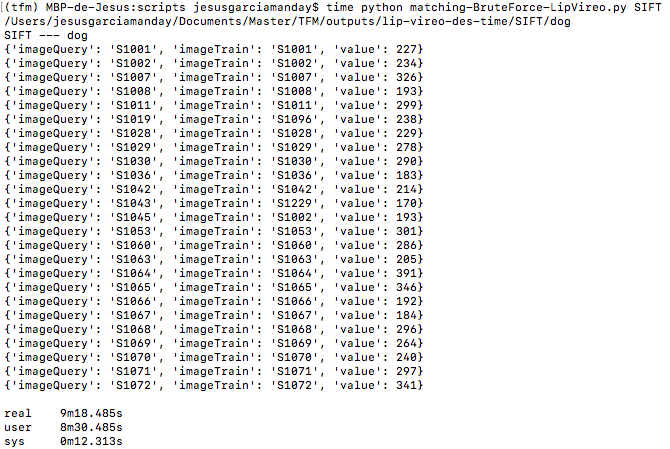
\includegraphics[width=130mm]{tfm-img83}}
\caption{Tiempo empleado para calcular la distancia entre los puntos de interés del subconjunto seleccionado.} \label{fig:señales}
\end{figure} 

\vspace{100mm}

Para mejorar estos resultados debido a la enorme cantidad y variedad de pruebas que se tienen que realizar por cada diferente escenario y que conllevarían un largo periodo de tiempo en computación, se propone emplear una nueva alternativa que mejore los tiempos de rendimiento para poder así agilizar en las diferentes experimentaciones. \\

Para ello se va a utilizar un algoritmo basado en Flann (Fast Library for Approximate Nearest Neighbors). Este tipo de algoritmo emplea la misma metodología para la comparación de características que el método anterior, es decir, el cálculo de distancias entre puntos. La diferencia entre ambos radica en que Flann no realiza el matching de todos los puntos de una imagen A con todos los puntos de imagen B, sino que en vez de eso trabaja con una estructura de árbol kd que es usada para la búsqueda del vecino más cercano. La principal ventaja de usar Flann es que para conjuntos de datos amplios es mucho más rapido que BruteForce debido a que trabaja internamente con árboles dimensionales, lo que permite reducir el tiempo de cómputo. \\

El uso de este algoritmo para la comparación es simplemente para disminuir el tiempo de cómputo empleado, ya que los resultados que arroje serán los mismos que se obtienen con BruteForce ya que ambos implementan la misma metodología para el cálculo de la distancia. \\

Se han realizado una serie de experimentaciones para comparar el tiempo empledo por cada método para varios subconjuntos de imágenes del 25\%, 30\%, 40\% y 45\% sobre el conjunto total de las mismas. Los resultados que se han obtenido se muestran el figura siguiente:




\begin{figure}[htbp]
\centering
\subfigure{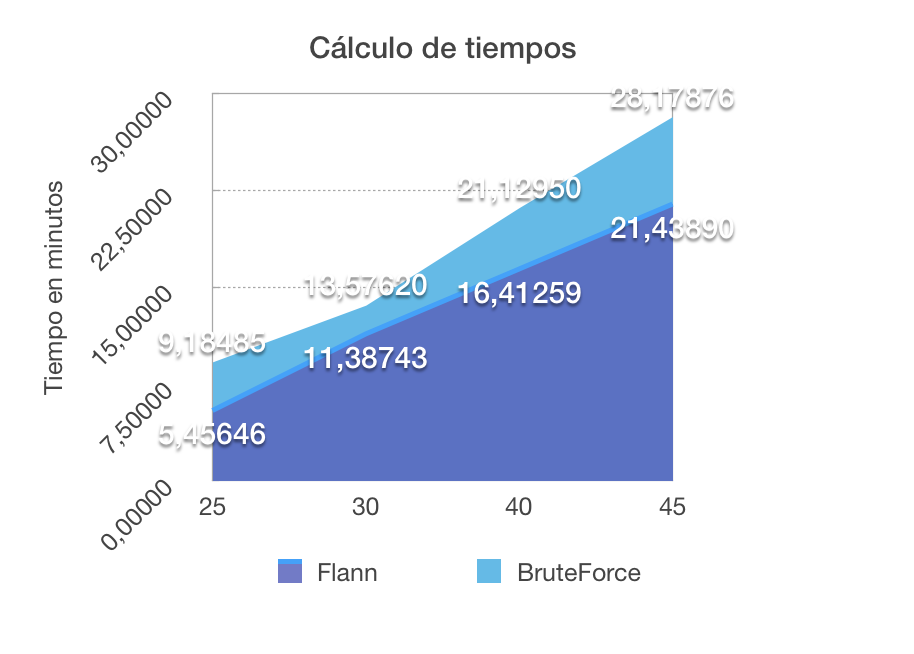
\includegraphics[width=130mm]{tfm-img86}}
\caption{Tiempo empleado para calcular la distancia entre los puntos de interés para el 25\%, 30\%, 40\%, y 45\%.} \label{fig:señales}
\end{figure} 

\newpage

En la gráfica anterior se puede observar como el tiempo de cómputo disminuye con Flann a medida que el conjunto de datos va aumentando. 


\subsection{Método de fusión de detectores de puntos de interés propuesto}
Como se viene indicando a lo largo de esta memoria, una de las aportaciones que desde este Trabajo Fin de Master se quiere hacer en el campo de la investigación de los sistemas de reconocimiento basados en el iris en condiciones no ideales, es la de definir una nueva alternativa para la detección de los puntos de interés sobre una imagen de iris en el espacio de escala. \\

La base fundamental de esta propuesta parte de la premisa de que conociendo los buenos resultados que arrojan cada uno de los detectores de puntos de interés mencionados anteriormente sobre una imagen de iris, podemos suponer entonces que realizando una correcta fusión de los mismos los resultados tendrían que mejorar a los que se obtienen utilizándolos individualmente. \\

El esquema de fusión propuesto está basado en una regla de suma ponderada de las puntuaciones obtenidas por las 3 fuentes de información (Harris-Laplace, Hessian-Laplace y Fast-Hessian). Debido a la naturaleza homogénea de las fuentes de puntuaciones empleadas, no se precisa de la ejecución de ningún proceso de normalización previo a realizar la fusión de las mismas. Para obtener las ponderaciones de cada una de las fuentes se sigue un esquema basado en el ranking de las mismas mediante sus medidas de desempeño. Dicho esquema surge de la suposición de que la fuente más fiable es aquella que mejor satisface los objetivos que se plantean en un contexto específico. De este modo, se asume que la fuente que mejor satisface un objetivo recibe el valor más alto en el ranking el cual se corresponde con el número de fuentes n. Por otro lado, la fuente que menos satisface un objetivo recibe el menor valor del ranking, siendo la posición 1. \\

Finalmente, la ponderación correspondiente a una fuente viene dada por la proporción de su ranking acumulado respecto al total de rankings acumulados por las n fuentes. \\

En cuanto a la fusión de las 3 fuentes de detectores de puntos de interés para reconocimiento de iris, se propone la utilización de medidas de desempeño del reconocimiento con las fuentes individuales como objetivos a satisfacer para calcular su rendimiento. Uno de los objetivos que se plantea es la maximización de la AUC (en inglés "area under the curve"). La AUC o Curva de ROC es una representación gráfica que muestra la sensibilidad frente a la especifidad para un sistema clasificatorio, llevado a este contexto, representa la sensibilidad en función de los falsos positivos para distintos puntos de corte. Otro de los objetivos empleados como medida de desempeño es el valor ERR (en inglés "equal error rate"), el cual se obtiene como resultado del tipo de curva cosechado anteriormente, representando una medida de gran importancia ya que nos va a indicar la tasa de error. El último de los objetivos que se va utilizar es el CRR (en inglés "correct recognition rate"). Esta media representa el tanto por ciento de veces en que la correcta identidad de un individuo presentado  ante el sistema aparece entre las primeras k identidades.  \\


\subsubsection{Análisis de las medidas de desempeño sobre las fuentes de información }
Para la selección de los tres detectores mencionados (Harris-Laplace, Hessian-Laplace y Fast-Hessian) que formarán el método de fusión propuesto, se siguió un esquema basado en la suma ponderada de medidas de desempeño obtenidas por cada uno de los detectores de manera individual (Dense, DoG, Harris-Laplace, Hessian-Laplace, Harris, Hessian, Fast-Hessian (SURF) y Log) sobre los objetivos AUC y EER, de manera que se buscará los valores máximos para el AUC y los valores mínimos para el ERR. 

Con la base de datos de imágenes previamente establecida (CASIA-IrisV4-Interval), la cual proporciona 2639 imágenes de 249 individuos con diferentes factores de calidad adheridos, se ha decidido clasificarla en función del nivel de afectación que posee cada una de las imágenes. Claramente, se ha podido observar que el global de las imágenes las podemos clasificar en 3 subconjuntos dependiendo del tipo de factor de calidad que tenga, de este modo tenemos un primer conjunto de imágenes afectadas por reflexión especular (1247), un segundo conjunto de imágenes afectadas por iluminación variable (852) y un último conjunto de imágenes afectadas por oclusión de párpados y pestañas (540). \\

Cada una de las medidas de desempeño se aplicará sobre cada uno de los subconjuntos de las imágenes, viendo así como afecta el grado de calidad de la imagen tanto a cada uno de los detectores mencionados. Estas pruebas se han realizado en una máquina en el que se ha realizado la que consta de unas características basadas en un procesador Intel Core i5 a 2 GHz, 8 GB  de memoria RAM LPDDR3 a 1867 MHz y un disco duro con una capacidad de 256 GB SSD. \\

Se ha usado validación cruzada con un 80\% de los ejemplos para el entrenamiento y un 20\% para test. En la imagen siguiente se exponen los resultados. \\

\begin{table}[h]
\begin{center}
\begin{tabular}{@{}lccc@{}}
\toprule
&& Casia-IrisV4-Interval & \\ \hline
&Reflexión especular		&  	Iluminación variable		& Oclusión \\ \hline
&AUC  \phantom{aa} EER  &  	AUC  \phantom{aa} EER 	& AUC  \phantom{aa} EER  \\ \hline
Dense& 91.32 \phantom{aa} 9.78   &  	90.23 \phantom{aa} 11.68  & 91.61 \phantom{aa} 9.59  \\
Dog& 93.56 \phantom{aa} 7.78   &  	92.87 \phantom{aa} 7.31  & 93.45 \phantom{aa} 7.21  \\
Harris-Laplace& 96.93 \phantom{aa} 5.76   &  	96.02 \phantom{aa} 5.89  & 97.58 \phantom{aa} 3.88  \\
Hessian-Laplace& 96.73 \phantom{aa} 5.11   &  95.34 \phantom{aa} 5.56 & 96.12 \phantom{aa} 5.21  \\
Harris& 95.21  \phantom{aa}5.04  &  	94.36 \phantom{aa} 4.90  & 94.07  \phantom{aa}5.82  \\
Hessian& 94.70 \phantom{aa} 6.43   &  95.21 \phantom{aa} 5.74  & 95.14 \phantom{aa} 5.81  \\
Log& 94.78 \phantom{aa} 6.12  &  94.24  \phantom{aa}5.77 & 95.32 \phantom{aa} 5.15   \\ 
Fast-Hessian& 97.23 \phantom{aa} 3.54   &  	96.54 \phantom{aa} 4.50  & 97.31 \phantom{aa} 4.33  \\

\end{tabular}
\end{center}
\caption{Medidas de desempeño del reconocimiento sobre los subconjuntos de imágenes utilizando cada una de las fuentes individuales.}
\label{my_tabla}
\end{table}


Como se puede observar por los valores arrojados en las diferentes medidas de desempeño en esta primera prueba, las fuentes \textbf{Harris-Laplace}, \textbf{Hessian-Laplace} y \textbf{Fast-Hessian} son las que han obtenido los mayores valores para el objetivo AUC, y los valores mínimos para el objetivo ERR en cada uno de los conjuntos de imágenes. Para eliminar el factor de la aleatoriedad que puede llegar a incidir en los resultados de las medidas de desempeño, se han vuelto a repetir las pruebas varias veces volviendo a seleccionar otro 20\% de imágenes de los diferentes subconjuntos en cada una de ellas para la posterior validación cruzada. \\ 


\begin{table}[h]
\begin{center}
\begin{tabular}{@{}lccc@{}}
\toprule
&& Casia-IrisV4-Interval & \\ \hline
&Reflexión especular		&  	Iluminación variable		& Oclusión \\ \hline
&AUC  \phantom{aa} EER  &  	AUC  \phantom{aa} EER 	& AUC  \phantom{aa} EER  \\ \hline
Dense& 91.66 \phantom{aa} 9.39   &  	90.72 \phantom{aa} 11.16  & 90.98 \phantom{aa} 10.23  \\
Dog& 93.13 \phantom{aa} 7.31   &  	92.67 \phantom{aa} 7.08  & 93.87 \phantom{aa} 7.42  \\
Harris-Laplace& 97.12 \phantom{aa} 5.22   &  	96.23 \phantom{aa} 5.54  & 97.65 \phantom{aa} 3.29  \\
Hessian-Laplace& 96.13 \phantom{aa} 5.21   &  95.01 \phantom{aa} 5.17 & 96.74 \phantom{aa} 5.10  \\
Harris& 94.76  \phantom{aa}5.23  &  	94.12 \phantom{aa} 5.37  & 94.91  \phantom{aa}5.93  \\
Hessian& 94.35 \phantom{aa} 6.32   &  94.73 \phantom{aa} 5.66  & 94.37 \phantom{aa} 5.89  \\
Log& 94.13 \phantom{aa} 6.53  &  94.10  \phantom{aa}5.90 & 95.41 \phantom{aa} 5.87   \\ 
Fast-Hessian& 97.33 \phantom{aa} 3.43   &  	96.88 \phantom{aa} 4.76  & 97.38 \phantom{aa} 4.75  \\

\end{tabular}
\end{center}
\caption{Medidas de desempeño del reconocimiento sobre los subconjuntos de imágenes utilizando cada una de las fuentes individuales (II).}
\label{my_tabla}
\end{table}


\begin{table}[h]
\begin{center}
\begin{tabular}{@{}lccc@{}}
\toprule
&& Casia-IrisV4-Interval & \\ \hline
&Reflexión especular		&  	Iluminación variable		& Oclusión \\ \hline
&AUC  \phantom{aa} EER  &  	AUC  \phantom{aa} EER 	& AUC  \phantom{aa} EER  \\ \hline
Dense& 91.12 \phantom{aa} 9.43   &  	90.45 \phantom{aa} 11.01  & 91.07 \phantom{aa} 10.01  \\
Dog& 93.57 \phantom{aa} 7.22   &  	92.35 \phantom{aa} 7.49  & 93.20 \phantom{aa} 7.34  \\
Harris-Laplace& 97.34 \phantom{aa} 5.01   &  	96.75 \phantom{aa} 5.12  & 97.78 \phantom{aa} 3.33  \\
Hessian-Laplace& 96.24 \phantom{aa} 5.21   &  95.74 \phantom{aa} 5.11 & 96.67 \phantom{aa} 5.19  \\
Harris& 94.19  \phantom{aa}5.73  &  	94.54 \phantom{aa} 5.66  & 94.75  \phantom{aa}5.68  \\
Hessian& 94.73 \phantom{aa} 6.13   &  95.61 \phantom{aa} 5.23  & 95.63 \phantom{aa} 5.54  \\
Log& 94.54 \phantom{aa} 6.21  &  94.75  \phantom{aa}5.12 & 95.76 \phantom{aa} 5.21   \\ 
Fast-Hessian& 97.55 \phantom{aa} 3.26   &  	96.75 \phantom{aa} 4.54  & 97.59 \phantom{aa} 4.51  \\  \\  \\ 

\end{tabular}
\end{center}
\caption{Medidas de desempeño del reconocimiento sobre los subconjuntos de imágenes utilizando cada una de las fuentes individuales (III).}
\label{my_tabla}
\end{table} 

\newpage

\begin{table}[h]
\begin{center}
\begin{tabular}{@{}lccc@{}}
\toprule
&& Casia-IrisV4-Interval & \\ \hline
&Reflexión especular		&  	Iluminación variable		& Oclusión \\ \hline
&AUC  \phantom{aa} EER  &  	AUC  \phantom{aa} EER 	& AUC  \phantom{aa} EER  \\ \hline
Dense& 90.32 \phantom{aa} 9.89   &  	90.31 \phantom{aa} 10.75  & 91.21 \phantom{aa} 10.25  \\
Dog& 93.11 \phantom{aa} 7.93   &  	92.10 \phantom{aa} 8.01  & 93.82 \phantom{aa} 7.77  \\
Harris-Laplace& 97.81 \phantom{aa} 4.80   &  	96.23 \phantom{aa} 5.74  & 97.71 \phantom{aa} 3.37  \\
Hessian-Laplace& 96.44 \phantom{aa} 5.11   &  95.81 \phantom{aa} 5.36 & 96.01 \phantom{aa} 5.48  \\
Harris& 94.29  \phantom{aa}5.32  &  	94.12 \phantom{aa} 5.89  & 94.87  \phantom{aa}6.11  \\
Hessian& 94.12 \phantom{aa} 6.41   &  94.83 \phantom{aa} 5.97  & 95.37 \phantom{aa} 5.74  \\
Log& 94.31 \phantom{aa} 6.38  &  94.13  \phantom{aa}5.83 & 95.01 \phantom{aa} 5.89   \\ 
Fast-Hessian& 97.35 \phantom{aa} 3.12   &  	96.81 \phantom{aa} 4.41  & 97.70 \phantom{aa} 4.34  \\  \\  \\

\end{tabular}
\end{center}
\caption{Medidas de desempeño del reconocimiento sobre los subconjuntos de imágenes utilizando cada una de las fuentes individuales (IV).}
\label{my_tabla}
\end{table}


\begin{table}[h]
\begin{center}
\begin{tabular}{@{}lccc@{}}
\toprule
&& Casia-IrisV4-Interval & \\ \hline
&Reflexión especular		&  	Iluminación variable		& Oclusión \\ \hline
&AUC  \phantom{aa} EER  &  	AUC  \phantom{aa} EER 	& AUC  \phantom{aa} EER  \\ \hline
Dense& 92.01 \phantom{aa} 8.23   &  	91.01 \phantom{aa} 10.12  & 91.32 \phantom{aa} 10.34  \\
Dog& 93.11 \phantom{aa} 7.82   &  	92.23 \phantom{aa} 7.33  & 92.14 \phantom{aa} 8.45  \\
Harris-Laplace& 97.67 \phantom{aa} 5.12   &  	96.01 \phantom{aa} 5.63  & 96.98 \phantom{aa} 3.45  \\
Hessian-Laplace& 96.12 \phantom{aa} 5.73   &  95.89 \phantom{aa} 5.08 & 97.71 \phantom{aa} 5.21  \\
Harris& 94.24  \phantom{aa}5.63  &  	93.32 \phantom{aa} 6.16  & 94.34  \phantom{aa}5.72  \\
Hessian& 94.69 \phantom{aa} 6.23   &  95.17 \phantom{aa} 5.38  & 94.15 \phantom{aa} 6.12  \\
Log& 94.11 \phantom{aa} 6.91  &  94.01  \phantom{aa}5.78 & 94.71 \phantom{aa} 5.87   \\ 
Fast-Hessian& 97.17 \phantom{aa} 3.34   &  	97.00 \phantom{aa} 4.01  & 97.61 \phantom{aa} 4.24  \\  \\  \\

\end{tabular}
\end{center}
\caption{Medidas de desempeño del reconocimiento sobre los subconjuntos de imágenes utilizando cada una de las fuentes individuales (V).}
\label{my_tabla}
\end{table}

\newpage

Tras haber realizado más pruebas sobre los mismos detectores y haber aplicado la validación cruzada sobre los resultados obtenidos, podemos observar como el resultado final sigue manteniendo la misma línea que los anteriores, siendo las fuentes de información de Harris-Laplace, Hessian-Laplace y Harris las que mejores medidas de desempeño han generado frente a los dos objetivos propuestos en los diferentes conjuntos de imágenes. \\

Además de que haya quedado claramente demostrado que esas tres fuentes de información son las que mejores resultados han aportado, también podemos ver otra serie de conclusiones verdaderamente importantes con respecto a estos resultados. Se puede observar como para imágenes con afectaciones por oclusión, el detector Harris-Laplace es el que mejores resultados ha obtenido. De igual modo, se puede deducir que para imágenes con afectaciones por reflexión especular la fuente de información Fast-Hessian es la que mejor rendimiento ha conseguido en cada uno de los objetivos. \\  \\  \\  \\


\subsubsection{Esquema de fusión }
Con las anteriores experimentaciones se ha podido comprobar que los 3 detectores propuestos para la fusión son los que mejores resultados han ofrecido frente al resto sobre los 3 diferentes conjuntos de imágenes disponibles. Dicho esto y con resultados expuestos en las anteriores figuras hemos realizado el esquema de fusión en base a las ponderaciones de las medidas de desempeño para cada uno de los objetivos empleados. \\

\begin{table}[h]
\begin{center}
\begin{tabular}{@{}lccccc@{}}
\toprule
&	&  	Reflexión especular		& &  \\ \hline
&Objetivo 1   &  Objetivo 2   & \( \gamma_{i} \) &  \( \omega{i} \) \\ \hline
Harris-Laplace& 2    &  3 & 5 & 0.42 \\
Hessian-Laplace& 1   &  2  & 3 & 0.25 \\
Fast-Hessian& 3  &  	1 & 4 & 0.33  \\ \hline
&   &  	 & 12 & 1  \\ \hline

\end{tabular}
\end{center}
\caption{Ponderaciones computadas sobre las 3 fuentes de interés con respecto a 2 objetivos para el conjunto de imágenes con reflexión especular.}
\label{my_tabla}
\end{table}

\begin{table}[h]
\begin{center}
\begin{tabular}{@{}lccccc@{}}
\toprule
&	&  	Iluminación variable		& &  \\ \hline
&Objetivo 1   &  Objetivo 2   & \( \gamma_{i} \) &  \( \omega{i} \) \\ \hline
Harris-Laplace& 2    &  1 & 3 & 0.25 \\
Hessian-Laplace& 1   &  3  & 4 & 0.33 \\
Fast-Hessian& 3  &  	2 & 5 & 0.42  \\ \hline
&   &  	 & 12 & 1  \\ \hline

\end{tabular}
\end{center}
\caption{Ponderaciones computadas sobre las 3 fuentes de interés con respecto a 2 objetivos para el conjunto de imágenes con iluminación variable.}
\label{my_tabla}
\end{table}

\begin{table}[h]
\begin{center}
\begin{tabular}{@{}lccccc@{}}
\toprule
&	&  	Oclusión		& &  \\ \hline
&Objetivo 1   &  Objetivo 2   & \( \gamma_{i} \) &  \( \omega{i} \) \\ \hline
Harris-Laplace& 3    &  1 & 4 & 0.33 \\
Hessian-Laplace& 1   &  2  & 3 & 0.25 \\
Fast-Hessian& 2  &  	3 & 5 & 0.42  \\ \hline
&   &  	 & 12 & 1  \\ \hline

\end{tabular}
\end{center}
\caption{Ponderaciones computadas sobre las 3 fuentes de interés con respecto a 2 objetivos para el conjunto de imágenes con oclusión.}
\label{my_tabla}
\end{table}

Como se puede apreciar, para cada uno de los subconjuntos de imágenes cada fuente de información ha obtenido su correspondiente ponderaración para la fusión, de manera que estos serán aplicados para realizar la extracción de las características. Esto quiere decir que la fusión de los 3 detectores de puntos de interés serán ponderada en base al tipo de imagen, y de cada una de ellas se obtendrá un porcentaje de las características de una imagen. \\

\subsubsection{Análisis de las medidas de desempeño en la fusión }
Una vez definido el esquema de fusión, lo siguiente es comprobar el grado de robustez y precisión que tendría la fusión de dichos métodos en comparación con cada uno de ellos de manera individual.  Para ello, se va a realizar el esquema de puntuaciones mencionado al comienzo de este punto donde se ponderarán las medidas de desempeño obtenidas por cada una de las fuentes individualmente y en conjunto. En este escenario se tomarán los 3 objetivos descritos para generar dichas medidas a diferencia del escenario anterior. Al igual que antes, se usará validación cruzada con un 80\% de los ejemplos para entrenamiento y un 20\% para test. En el cuadro de abajo se muestran los resultados obtenidos. \\ \\ \\ \\ \\ \\ 


\begin{table}[h]
\begin{center}
\begin{tabular}{@{}lccc@{}}
\toprule
&& Casia-IrisV4-Interval & \\ \hline
&Reflexión especular		&  	Iluminación variable		& Oclusión \\ \hline
&AUC  \phantom{aa} EER  \phantom{aa} CRR &  	AUC  \phantom{aa} EER  \phantom{aa} CRR		& AUC  \phantom{aa} EER  \phantom{aa} CRR \\ \hline
Harris-Laplace& 97.32 \phantom{aa} 3.40  \phantom{aa} 96.81 &  	96.11 \phantom{aa} 4.70  \phantom{aa}97.12		& 97.33 \phantom{aa} 4.61 \phantom{aa} 96.14 \\
Hessian-Laplace& 96.70 \phantom{aa} 5.32  \phantom{aa} 96.15 &  	95.21 \phantom{aa} 5.22 \phantom{aa} 95.77 & 96.01 \phantom{aa} 5.41 \phantom{aa} 95.22 \\
Fast-Hessian& 98.20  \phantom{aa}3.04 \phantom{aa}  97.26 &  	98.36 \phantom{aa} 4.40  \phantom{aa}97.71		& 98.17  \phantom{aa}3.82 \phantom{aa} 98.11 \\
Fusión& 99.12 \phantom{aa} 2.57  \phantom{aa}98.18 &  	98.88  \phantom{aa}3.15 \phantom{aa} 98.02		& 99.21 \phantom{aa} 2.82  \phantom{aa}98.77 \\ \hline

\end{tabular}
\end{center}
\caption{Medidas de desempeño del reconocimiento sobre los conjuntos de imágenes utilizando las fuentes individuales y la fusión de las mismas.}
\label{my_tabla}
\end{table}


Observando los valores arrojados en las diferentes medidas de desempeño, se puede comprobar como la opción de fusión de ambos métodos ha obtenido los valores máximos para los objetivos AUC y CRR, y el valor mínimo para el objetivo ERR en cada uno de los subconjuntos de imágenes. Del mismo modo que se hizo y para eliminar el factor de la aleatoriedad presente, se han vuelto a repetir las pruebas varias veces volviendo a seleccionar otro 20\% de imágenes de los diferentes conjuntos en cada una de ellas para la posterior validación cruzada. \\

\begin{table}[h]
\begin{center}
\begin{tabular}{@{}lccc@{}}
\toprule
&& Casia-IrisV4-Interval & \\ \hline
&Reflexión especular		&  	Iluminación variable		& Oclusión \\ \hline
&AUC  \phantom{aa} EER  \phantom{aa} CRR &  	AUC  \phantom{aa} EER  \phantom{aa} CRR		& AUC  \phantom{aa} EER  \phantom{aa} CRR \\ \hline
Harris-Laplace& 98.22 \phantom{aa} 3.11  \phantom{aa} 97.17 &  	97.53 \phantom{aa} 3.89  \phantom{aa}97.44		& 98.07 \phantom{aa} 4.21 \phantom{aa} 97.11 \\
Hessian-Laplace& 97.11 \phantom{aa} 5.43  \phantom{aa} 96.01 &  	96.07 \phantom{aa} 5.15 \phantom{aa} 95.98 & 96.32 \phantom{aa} 5.12 \phantom{aa} 95.85 \\
Fast-Hessian& 98.34  \phantom{aa}2.63 \phantom{aa}  97.88 &  	98.83 \phantom{aa} 3.86  \phantom{aa}98.23		& 98.14  \phantom{aa}3.68 \phantom{aa} 97.91 \\
Fusión& 99.44 \phantom{aa} 2.12  \phantom{aa}98.84 &  	99.33  \phantom{aa}2.48 \phantom{aa} 99.04		& 99.64 \phantom{aa} 2.58  \phantom{aa}99.09 \\ \hline

\end{tabular}
\end{center}
\caption{Medidas de desempeño del reconocimiento sobre los conjuntos de imágenes utilizando las fuentes individuales y la fusión de las mismas (II).}
\label{my_tabla}
\end{table}

\begin{table}[h]
\begin{center}
\begin{tabular}{@{}lccc@{}}
\toprule
&& Casia-IrisV4-Interval & \\ \hline
&Reflexión especular		&  	Iluminación variable		& Oclusión \\ \hline
&AUC  \phantom{aa} EER  \phantom{aa} CRR &  	AUC  \phantom{aa} EER  \phantom{aa} CRR		& AUC  \phantom{aa} EER  \phantom{aa} CRR \\ \hline
Harris-Laplace& 97.44 \phantom{aa} 3.21  \phantom{aa} 96.91 &  	96.18 \phantom{aa} 4.56  \phantom{aa}97.41		& 97.45 \phantom{aa} 4.49 \phantom{aa} 96.44 \\
Hessian-Laplace& 96.78 \phantom{aa} 5.25  \phantom{aa} 96.46 &  	95.43 \phantom{aa} 5.11 \phantom{aa} 95.90 & 96.70 \phantom{aa} 5.24 \phantom{aa} 95.72\\
Fast-Hessian& 98.45  \phantom{aa}2.94 \phantom{aa}  97.67 &  	98.57 \phantom{aa} 4.32 \phantom{aa}97.87		& 98.80  \phantom{aa}3.33 \phantom{aa} 98.56 \\
Fusión& 99.34 \phantom{aa} 2.22  \phantom{aa}98.31 &  	99.02  \phantom{aa}3.01 \phantom{aa} 98.83		& 99.76 \phantom{aa} 2.36  \phantom{aa}99.13 \\ \hline

\end{tabular}
\end{center}
\caption{Medidas de desempeño del reconocimiento sobre los conjuntos de imágenes utilizando las fuentes individuales y la fusión de las mismas (III).}
\label{my_tabla}
\end{table}

\newpage

\begin{table}[h]
\begin{center}
\begin{tabular}{@{}lccc@{}}
\toprule
&& Casia-IrisV4-Interval & \\ \hline
&Reflexión especular		&  	Iluminación variable		& Oclusión \\ \hline
&AUC  \phantom{aa} EER  \phantom{aa} CRR &  	AUC  \phantom{aa} EER  \phantom{aa} CRR		& AUC  \phantom{aa} EER  \phantom{aa} CRR \\ \hline
Harris-Laplace& 97.11 \phantom{aa} 3.65  \phantom{aa} 96.08 &  	95.24 \phantom{aa} 4.80  \phantom{aa}96.92		& 97.12 \phantom{aa} 4.93 \phantom{aa} 95.89 \\
Hessian-Laplace& 96.21 \phantom{aa} 5.75 \phantom{aa} 95.34 &  	95.10 \phantom{aa} 5.78 \phantom{aa} 94.09 & 95.49 \phantom{aa} 5.79 \phantom{aa} 95.03 \\
Fast-Hessian& 97.87  \phantom{aa}3.76 \phantom{aa}  96.78 &  	97.77 \phantom{aa} 4.85  \phantom{aa}97.10		& 97.65  \phantom{aa}4.01 \phantom{aa} 97.60 \\
Fusión& 98.99 \phantom{aa} 2.80  \phantom{aa}97.79 &  	98.13  \phantom{aa}3.54 \phantom{aa} 97.64		& 98.91 \phantom{aa} 2.98 \phantom{aa}98.12 \\   \hline

\end{tabular}
\end{center}
\caption{Medidas de desempeño del reconocimiento sobre los conjuntos de imágenes utilizando las fuentes individuales y la fusión de las mismas (IV).}
\label{my_tabla}
\end{table}


\begin{table}[h]
\begin{center}
\begin{tabular}{@{}lccc@{}}
\toprule
&& Casia-IrisV4-Interval & \\ \hline
&Reflexión especular		&  	Iluminación variable		& Oclusión \\ \hline
&AUC  \phantom{aa} EER  \phantom{aa} CRR &  	AUC  \phantom{aa} EER  \phantom{aa} CRR		& AUC  \phantom{aa} EER  \phantom{aa} CRR \\ \hline
Harris-Laplace& 97.34 \phantom{aa} 3.12  \phantom{aa} 96.43 &  	95.12 \phantom{aa} 4.72  \phantom{aa}96.63		& 97.78 \phantom{aa} 4.15 \phantom{aa} 95.77 \\
Hessian-Laplace& 96.32 \phantom{aa} 5.87 \phantom{aa} 95.14 &  	95.43 \phantom{aa} 5.87 \phantom{aa} 94.16 & 95.43 \phantom{aa} 5.43 \phantom{aa} 95.17 \\
Fast-Hessian& 97.67  \phantom{aa}3.54 \phantom{aa}  96.54 &  	97.33 \phantom{aa} 4.12  \phantom{aa}97.34		& 97.54  \phantom{aa}4.38 \phantom{aa} 97.49 \\
Fusión& 98.78 \phantom{aa} 2.92  \phantom{aa}97.81 &  	98.07  \phantom{aa}3.21 \phantom{aa} 97.72		& 98.88 \phantom{aa} 2.99 \phantom{aa}98.43 \\ \hline

\end{tabular}
\end{center}
\caption{Medidas de desempeño del reconocimiento sobre los conjuntos de imágenes utilizando las fuentes individuales y la fusión de las mismas (V).}
\label{my_tabla}
\end{table}


Viendo los resultados obtenidos en las medidas de desempeño sobre cada una de las iteraciones que se ha realizado y habiendo aplicado la validación cruzada los mismos, es en todos los casos el método de fusión el que mejores valores de maxímo y mínimo alcanza para los diferentes valores de objetivos. Vamos a continuar realizando algunas pruebas más sobre las medidas de desempeño variando en este caso la cantidad de imágenes seleccionadas a clasificar. Se van a realizar las mismas pruebas anteriores pero modificando a un 15\% y 25\% la cantidad de imágenes sobre las que se evaluará la medida de desempeño volviendo a aplicar la validación cruzada para cada uno de los supuestos.\\ 


\begin{table}[h]
\begin{center}
\begin{tabular}{@{}lccc@{}}
\toprule
&& Casia-IrisV4-Interval & \\ \hline
&Reflexión especular		&  	Iluminación variable		& Oclusión \\ \hline
&AUC  \phantom{aa} EER  \phantom{aa} CRR &  	AUC  \phantom{aa} EER  \phantom{aa} CRR		& AUC  \phantom{aa} EER  \phantom{aa} CRR \\ \hline
Harris-Laplace& 97.68 \phantom{aa} 3.14  \phantom{aa} 96.98 &  	96.23 \phantom{aa} 4.76  \phantom{aa}97.64		& 97.82 \phantom{aa} 4.17 \phantom{aa} 96.68 \\
Hessian-Laplace& 97.03 \phantom{aa} 5.15  \phantom{aa} 96.89 &  	95.64 \phantom{aa} 5.08 \phantom{aa} 96.10 & 96.81 \phantom{aa} 5.03 \phantom{aa} 95.98\\
Fast-Hessian& 98.79  \phantom{aa}2.56 \phantom{aa}  97.97 &  	98.78 \phantom{aa} 4.54 \phantom{aa}98.12		& 98.90  \phantom{aa}3.19 \phantom{aa} 98.87 \\
Fusión& 99.43 \phantom{aa} 2.15  \phantom{aa}98.56 &  	99.21  \phantom{aa}2.78 \phantom{aa} 98.97		& 99.87 \phantom{aa} 2.12  \phantom{aa}99.21 \\ \hline

\end{tabular}
\end{center}
\caption{Medidas de desempeño del reconocimiento sobre los conjuntos de imágenes utilizando las fuentes individuales y la fusión de las mismas sobre un 15\% de imágenes a clasificar .}
\label{my_tabla}
\end{table}

\begin{table}[h]
\begin{center}
\begin{tabular}{@{}lccc@{}}
\toprule
&& Casia-IrisV4-Interval & \\ \hline
&Reflexión especular		&  	Iluminación variable		& Oclusión \\ \hline
&AUC  \phantom{aa} EER  \phantom{aa} CRR &  	AUC  \phantom{aa} EER  \phantom{aa} CRR		& AUC  \phantom{aa} EER  \phantom{aa} CRR \\ \hline
Harris-Laplace& 97.34 \phantom{aa} 3.54  \phantom{aa} 96.87 &  	96.43 \phantom{aa} 4.56  \phantom{aa}97.32		& 97.65 \phantom{aa} 4.21 \phantom{aa} 96.72 \\
Hessian-Laplace& 97.12 \phantom{aa} 5.54  \phantom{aa} 96.81 &  	95.34 \phantom{aa} 5.16 \phantom{aa} 96.34 & 96.65 \phantom{aa} 5.33 \phantom{aa} 95.89\\
Fast-Hessian& 98.89  \phantom{aa}2.44 \phantom{aa}  97.71 &  	98.65 \phantom{aa} 4.35 \phantom{aa}98.34		& 98.75  \phantom{aa}3.33 \phantom{aa} 98.73 \\
Fusión& 99.14 \phantom{aa} 2.33  \phantom{aa}98.64 &  	99.33  \phantom{aa}2.67 \phantom{aa} 98.77		& 99.81 \phantom{aa} 2.21  \phantom{aa}99.19 \\ \hline

\end{tabular}
\end{center}
\caption{Medidas de desempeño del reconocimiento sobre los conjuntos de imágenes utilizando las fuentes individuales y la fusión de las mismas sobre un 15\% de imágenes a clasificar (II) .}
\label{my_tabla}
\end{table}

\newpage

\begin{table}[h]
\begin{center}
\begin{tabular}{@{}lccc@{}}
\toprule
&& Casia-IrisV4-Interval & \\ \hline
&Reflexión especular		&  	Iluminación variable		& Oclusión \\ \hline
&AUC  \phantom{aa} EER  \phantom{aa} CRR &  	AUC  \phantom{aa} EER  \phantom{aa} CRR		& AUC  \phantom{aa} EER  \phantom{aa} CRR \\ \hline
Harris-Laplace& 97.21 \phantom{aa} 3.41  \phantom{aa} 96.71 &  	96.61 \phantom{aa} 4.66  \phantom{aa}97.82		& 97.78 \phantom{aa} 4.34 \phantom{aa} 96.81 \\
Hessian-Laplace& 97.54 \phantom{aa} 5.24  \phantom{aa} 96.61 &  	95.43 \phantom{aa} 5.33 \phantom{aa} 96.54 & 96.35 \phantom{aa} 5.32 \phantom{aa} 95.18\\
Fast-Hessian& 98.78  \phantom{aa}2.32 \phantom{aa}  97.61 &  	98.56 \phantom{aa} 4.31 \phantom{aa}98.13		& 98.81  \phantom{aa}3.22 \phantom{aa} 98.53 \\
Fusión& 99.21 \phantom{aa} 2.43  \phantom{aa}98.55 &  	99.71  \phantom{aa}2.43 \phantom{aa} 98.21		& 99.76 \phantom{aa} 2.34  \phantom{aa}99.20 \\ \hline

\end{tabular}
\end{center}
\caption{Medidas de desempeño del reconocimiento sobre los conjuntos de imágenes utilizando las fuentes individuales y la fusión de las mismas sobre un 15\% de imágenes a clasificar (III) .}
\label{my_tabla}
\end{table}

\begin{table}[h]
\begin{center}
\begin{tabular}{@{}lccc@{}}
\toprule
&& Casia-IrisV4-Interval & \\ \hline
&Reflexión especular		&  	Iluminación variable		& Oclusión \\ \hline
&AUC  \phantom{aa} EER  \phantom{aa} CRR &  	AUC  \phantom{aa} EER  \phantom{aa} CRR		& AUC  \phantom{aa} EER  \phantom{aa} CRR \\ \hline
Harris-Laplace& 96.91 \phantom{aa} 3.78  \phantom{aa} 96.12 &  	96.45 \phantom{aa} 4.83  \phantom{aa}97.23		& 97.11 \phantom{aa} 4.87 \phantom{aa} 96.37 \\
Hessian-Laplace& 97.81 \phantom{aa} 5.34  \phantom{aa} 96.73 &  	95.54 \phantom{aa} 5.63 \phantom{aa} 96.73 & 96.31 \phantom{aa} 5.34 \phantom{aa} 96.17\\
Fast-Hessian& 98.23  \phantom{aa}2.34 \phantom{aa}  97.36 &  	98.71 \phantom{aa} 4.63 \phantom{aa}98.21		& 98.56  \phantom{aa}3.35 \phantom{aa} 98.73 \\
Fusión& 99.08 \phantom{aa} 2.32  \phantom{aa}98.36 &  	99.72  \phantom{aa}2.29 \phantom{aa} 98.11		& 99.56 \phantom{aa} 2.31  \phantom{aa}99.61 \\ \hline

\end{tabular}
\end{center}
\caption{Medidas de desempeño del reconocimiento sobre los conjuntos de imágenes utilizando las fuentes individuales y la fusión de las mismas sobre un 15\% de imágenes a clasificar (IV) .}
\label{my_tabla}
\end{table}


\begin{table}[h]
\begin{center}
\begin{tabular}{@{}lccc@{}}
\toprule
&& Casia-IrisV4-Interval & \\ \hline
&Reflexión especular		&  	Iluminación variable		& Oclusión \\ \hline
&AUC  \phantom{aa} EER  \phantom{aa} CRR &  	AUC  \phantom{aa} EER  \phantom{aa} CRR		& AUC  \phantom{aa} EER  \phantom{aa} CRR \\ \hline
Harris-Laplace& 96.43 \phantom{aa} 3.43  \phantom{aa} 96.21 &  	96.77 \phantom{aa} 4.72  \phantom{aa}97.34		& 97.31 \phantom{aa} 4.73 \phantom{aa} 96.31 \\
Hessian-Laplace& 97.66 \phantom{aa} 5.21  \phantom{aa} 96.81 &  	95.52 \phantom{aa} 5.54 \phantom{aa} 96.77 & 96.34 \phantom{aa} 5.13 \phantom{aa} 96.54\\
Fast-Hessian& 98.18  \phantom{aa}2.78 \phantom{aa}  97.44 &  	98.79 \phantom{aa} 4.56 \phantom{aa}98.37		& 98.71  \phantom{aa}3.43 \phantom{aa} 98.64 \\
Fusión& 99.19 \phantom{aa} 2.29  \phantom{aa}98.54 &  	99.35  \phantom{aa}2.34 \phantom{aa} 98.43		& 99.33 \phantom{aa} 2.23  \phantom{aa}99.44 \\ \hline

\end{tabular}
\end{center}
\caption{Medidas de desempeño del reconocimiento sobre los conjuntos de imágenes utilizando las fuentes individuales y la fusión de las mismas sobre un 15\% de imágenes a clasificar (V) .}
\label{my_tabla}
\end{table}

\newpage

\begin{table}[h]
\begin{center}
\begin{tabular}{@{}lccc@{}}
\toprule
&& Casia-IrisV4-Interval & \\ \hline
&Reflexión especular		&  	Iluminación variable		& Oclusión \\ \hline
&AUC  \phantom{aa} EER  \phantom{aa} CRR &  	AUC  \phantom{aa} EER  \phantom{aa} CRR		& AUC  \phantom{aa} EER  \phantom{aa} CRR \\ \hline
Harris-Laplace& 97.76 \phantom{aa} 3.13  \phantom{aa} 97.02 &  	96.67 \phantom{aa} 4.10  \phantom{aa}97.78		& 97.80 \phantom{aa} 4.13 \phantom{aa} 96.75 \\
Hessian-Laplace& 96.89 \phantom{aa} 5.10  \phantom{aa} 96.78 &  	95.78 \phantom{aa} 5.01 \phantom{aa} 96.12 & 96.98 \phantom{aa} 5.11 \phantom{aa} 95.98\\
Fast-Hessian& 98.76  \phantom{aa}2.60 \phantom{aa}  97.79 &  	99.04 \phantom{aa} 4.16 \phantom{aa}97.90		& 99.06  \phantom{aa}3.16 \phantom{aa} 98.94 \\
Fusión& 99.56 \phantom{aa} 2.12  \phantom{aa}98.80 &  	99.25  \phantom{aa}2.79 \phantom{aa} 98.91		& 99.85 \phantom{aa} 2.16  \phantom{aa}99.20 \\ \hline

\end{tabular}
\end{center}
\caption{Medidas de desempeño del reconocimiento sobre los conjuntos de imágenes utilizando las fuentes individuales y la fusión de las mismas sobre un 25\% de imágenes a clasificar.}
\label{my_tabla}
\end{table}

\begin{table}[h]
\begin{center}
\begin{tabular}{@{}lccc@{}}
\toprule
&& Casia-IrisV4-Interval & \\ \hline
&Reflexión especular		&  	Iluminación variable		& Oclusión \\ \hline
&AUC  \phantom{aa} EER  \phantom{aa} CRR &  	AUC  \phantom{aa} EER  \phantom{aa} CRR		& AUC  \phantom{aa} EER  \phantom{aa} CRR \\ \hline
Harris-Laplace& 97.13 \phantom{aa} 3.54  \phantom{aa} 97.52 &  	96.23 \phantom{aa} 4.33  \phantom{aa}97.43		& 97.90 \phantom{aa} 4.03 \phantom{aa} 97.01 \\
Hessian-Laplace& 96.65 \phantom{aa} 5.33  \phantom{aa} 96.54 &  	95.31 \phantom{aa} 5.33 \phantom{aa} 96.82 & 96.77 \phantom{aa} 5.22 \phantom{aa} 95.34\\
Fast-Hessian& 98.75  \phantom{aa}2.56 \phantom{aa}  97.81 &  	99.11 \phantom{aa} 4.23 \phantom{aa}97.43		& 99.33  \phantom{aa}3.29 \phantom{aa} 98.03 \\
Fusión& 99.51 \phantom{aa} 2.10  \phantom{aa}98.73 &  	99.33  \phantom{aa}2.91 \phantom{aa} 98.88		& 99.79 \phantom{aa} 2.43  \phantom{aa}99.50 \\ \hline

\end{tabular}
\end{center}
\caption{Medidas de desempeño del reconocimiento sobre los conjuntos de imágenes utilizando las fuentes individuales y la fusión de las mismas sobre un 25\% de imágenes a clasificar (II).}
\label{my_tabla}
\end{table}

\begin{table}[h]
\begin{center}
\begin{tabular}{@{}lccc@{}}
\toprule
&& Casia-IrisV4-Interval & \\ \hline
&Reflexión especular		&  	Iluminación variable		& Oclusión \\ \hline
&AUC  \phantom{aa} EER  \phantom{aa} CRR &  	AUC  \phantom{aa} EER  \phantom{aa} CRR		& AUC  \phantom{aa} EER  \phantom{aa} CRR \\ \hline
Harris-Laplace& 97.29 \phantom{aa} 3.22  \phantom{aa} 96.88 &  	96.31 \phantom{aa} 4.88  \phantom{aa}97.43		& 97.25 \phantom{aa} 4.54 \phantom{aa} 97.33 \\
Hessian-Laplace& 96.71 \phantom{aa} 5.43  \phantom{aa} 96.54 &  	95.83 \phantom{aa} 5.12 \phantom{aa} 96.54 & 96.73 \phantom{aa} 5.33 \phantom{aa} 95.78\\
Fast-Hessian& 98.67  \phantom{aa}2.44 \phantom{aa}  97.43 &  	99.21 \phantom{aa} 4.17 \phantom{aa}97.21		& 99.65  \phantom{aa}3.21 \phantom{aa} 98.34 \\
Fusión& 99.44 \phantom{aa} 2.39  \phantom{aa}98.56 &  	99.31  \phantom{aa}2.88 \phantom{aa} 98.73		& 99.67 \phantom{aa} 2.55  \phantom{aa}99.37 \\ \hline

\end{tabular}
\end{center}
\caption{Medidas de desempeño del reconocimiento sobre los conjuntos de imágenes utilizando las fuentes individuales y la fusión de las mismas sobre un 25\% de imágenes a clasificar (III).}
\label{my_tabla}
\end{table}

\newpage

\begin{table}[h]
\begin{center}
\begin{tabular}{@{}lccc@{}}
\toprule
&& Casia-IrisV4-Interval & \\ \hline
&Reflexión especular		&  	Iluminación variable		& Oclusión \\ \hline
&AUC  \phantom{aa} EER  \phantom{aa} CRR &  	AUC  \phantom{aa} EER  \phantom{aa} CRR		& AUC  \phantom{aa} EER  \phantom{aa} CRR \\ \hline
Harris-Laplace& 96.89 \phantom{aa} 3.43  \phantom{aa} 97.34 &  	96.43 \phantom{aa} 4.33  \phantom{aa}97.55		& 97.11 \phantom{aa} 4.83 \phantom{aa} 97.43 \\
Hessian-Laplace& 96.10 \phantom{aa} 5.32  \phantom{aa} 96.67 &  	95.12 \phantom{aa} 5.24 \phantom{aa} 96.33 & 96.65 \phantom{aa} 5.46 \phantom{aa} 95.81\\
Fast-Hessian& 98.65  \phantom{aa}2.36 \phantom{aa}  97.88 &  	99.31 \phantom{aa} 4.01 \phantom{aa}97.54		& 99.12  \phantom{aa}3.54 \phantom{aa} 98.65 \\
Fusión& 99.34 \phantom{aa} 2.66  \phantom{aa}98.64 &  	99.43  \phantom{aa}2.76 \phantom{aa} 98.43		& 99.21 \phantom{aa} 2.76  \phantom{aa}99.43 \\ \hline

\end{tabular}
\end{center}
\caption{Medidas de desempeño del reconocimiento sobre los conjuntos de imágenes utilizando las fuentes individuales y la fusión de las mismas sobre un 25\% de imágenes a clasificar (IV).}
\label{my_tabla}
\end{table}

\begin{table}[h]
\begin{center}
\begin{tabular}{@{}lccc@{}}
\toprule
&& Casia-IrisV4-Interval & \\ \hline
&Reflexión especular		&  	Iluminación variable		& Oclusión \\ \hline
&AUC  \phantom{aa} EER  \phantom{aa} CRR &  	AUC  \phantom{aa} EER  \phantom{aa} CRR		& AUC  \phantom{aa} EER  \phantom{aa} CRR \\ \hline
Harris-Laplace& 96.34 \phantom{aa} 3.54  \phantom{aa} 97.65 &  	96.12 \phantom{aa} 4.43  \phantom{aa}97.32		& 97.33 \phantom{aa} 4.54 \phantom{aa} 97.67 \\
Hessian-Laplace& 96.43 \phantom{aa} 5.41  \phantom{aa} 96.65 &  	95.54 \phantom{aa} 5.32 \phantom{aa} 96.43 & 96.54 \phantom{aa} 5.34 \phantom{aa} 95.77\\
Fast-Hessian& 98.43  \phantom{aa}2.43 \phantom{aa}  97.72 &  	99.44 \phantom{aa} 3.73 \phantom{aa}97.45		& 99.08  \phantom{aa}3.73 \phantom{aa} 98.57 \\
Fusión& 99.43 \phantom{aa} 2.54  \phantom{aa}98.34 &  	99.54  \phantom{aa}2.65 \phantom{aa} 98.51		& 99.23 \phantom{aa} 2.45  \phantom{aa}99.31 \\ \hline

\end{tabular}
\end{center}
\caption{Medidas de desempeño del reconocimiento sobre los conjuntos de imágenes utilizando las fuentes individuales y la fusión de las mismas sobre un 25\% de imágenes a clasificar (V).}
\label{my_tabla}
\end{table}

\newpage

Los resultados de estas últimas pruebas realizadas junto con los anteriores han vuelto a mostrar que la fusión de las 3 fuentes de información han obtenido las mejores puntuaciones en cada uno de los objetivos por cada subconjunto de imágenes. Este análisis destaca la mejora que la fusión de los 3 detectores ha conseguido frente a cada uno de ellos de manera indivual. Es por eso por lo que esta propuesta se postula como una alternativa fiable para la integración en los SRI. \\


%----------------------------------------------------------------------------------------